\section{Stetigkeit plus Zubehör (76-95)}
 
Definition der Stetigkeit von Funktionen, die auf Teilmengen der komplexen (oder reellen) Zahlen definiert sind und in die reellen oder komplexen Zahlen abbilden. Folgenkriterium für Stetigkeit. Sie sollten einfache Stetigkeitsbeweise sowohl mit dem Epsilon-Delta-Kriterium als auch mit dem Folgenkriterium durchföhren können. Satz: Sind zwei Funktionen stetig, so auch Vielfache, die Summe, das Produkt, der Quotient, falls der Nenner nicht Null ist, der Betrag der Funktion sowie der Realteil und der Imaginärteil der Funktion. Satz: Eine komplexwertige Funktion ist genau dann stetig, wenn ihr Realteil und ihr Imaginärteil beide stetig sind. Satz: Betragsfunktion, Polynome und rationale Funktionen sind stetig, sofern der Nenner nicht Null ist. Satz: Die Komposition stetiger Funktionen ist stetig. Definition von beschränkten, abgeschlossenen und kompakten Teilmengen der komplexen Zahlen. Beschränkte Intervalle sind beschränkt, abgeschlossene Intervalle sind abgeschlossen. Offene und halboffene Intervalle sind nicht abgeschlossen. Nur Intervalle der Form [a,b] sind kompakt. Epsilon-Umgebungen sind beschränkt, aber nicht abgeschlossen. Endliche Vereinigungen und beliebige Durchschnitte erhalten Beschränktheit, Abgeschlossenheit und Kompaktheit. Endliche Mengen sind kompakt. Urbilder von abgeschlossenen Mengen unter stetigen Abbildungen sind abgeschlossen. Abgeschlossene Kreisscheiben und Kreise sind kompakt. Halbräume in den komplexen Zahlen sind abgeschlossen. Satz: Stetige Bilder kompakter Mengen sind kompakt. Definition globaler und lokaler Extrema ((strenge) Minima und Maxima). Satz: Stetige Abbildungen auf kompakten Mengen nehmen ihr (globales) Maximum und Minimum an. Nullstellensatz von Bolzano, Zwischenwertsatz, stetige Funktionen bilden Intervalle auf Intervalle ab. Definition der n.ten Wurzel einer nichtnegativen Zahl; die zugehörige Funktion ist stetig und streng monoton steigend. Nicht rationale Zahlen heißen irrational; die Menge der rationalen Zahlen ist abzählbar; die Menge der irrationalen Zahlen ist nicht abzählbar. Definition der Dichtheit einer Menge in den reellen Zahlen. Satz: Die rationalen Zahlen sind dicht in den reellen Zahlen; die irrationalen Zahlen sind ebenfalls dicht. Satz: Jede reelle Zahl ist der Grenzwert einer streng steigenden Folge rationaler Zahlen und einer streng fallenden Folge rationaler Zahlen. Definition von Potenzen mit nichtnegativer Basis und reellen Exponenten; es gelten die üblichen Potenzgesetze. Definition von allgemeinen Potenzfunktionen und Exponentialfunktionen. Satz: Potenzfunktionen sind auf ihrem jeweiligen Definitionsbereich stetig, sowie streng steigend für positiven und streng fallend für negativen Exponenten. Satz: Exponentialfunktionen sind stetig sowie streng steigend für Basis a>1 und streng fallend für Basis 0 < a < 1. Definition des Logarithmus, speziell des natürlichen Logarithmus, Logarithmengesetze gemäß Th. 7.75. 


\subsection{Definition der Stetigkeit von Funktionen, die auf Teilmengen der komplexen (oder reellen) Zahlen definiert sind und in die reellen oder komplexen Zahlen abbilden (76)}

Let $M \subseteq \mathbb { C }$. If $\zeta \in M$, then a function $f : M \rightarrow \mathbb { K }$ is said to be
continuous in $\zeta$ if, and only if, for each $\epsilon > 0$, there is $\delta > 0$ such that the distance
between the values $f(z)$ and $f(\zeta)$ is less than $\epsilon$, provided the distance between $z$ and $\zeta$
is less than $\delta$, i.e. if, and only if,

\begin{align}
\underset{\epsilon \in \mathbb{R^+}}{\forall} \ \underset{\delta \in \mathbb{R^+}}{\exists} \ \underset{z \in M}{\forall} ( | z - \zeta | < \delta \Rightarrow | f ( z ) - f ( \zeta ) | < \epsilon ).
\end{align}

Moreover, $f$ is called continuous if, and only if, $f$ is continuous in every $\zeta \in M$. The set of
all continuous functions from $f : M \rightarrow \mathbb { K }$ is denoted by $C ( M ,\mathbb { K } )$, $C(M) := C(M,\mathbb{R})$.

\subsection{Folgenkriterium für Stetigkeit (78)}

Let $M \subseteq \mathbb { C }$, $f : M \rightarrow \mathbb { K }$. If $\zeta \in M$, then $f$ is continuous in $\zeta$ if, and only if, for each sequence $\left( z _ { n } \right) _ { n \in N }$ in $M$ with $\lim _ { n \rightarrow \infty } z _ { n } = \zeta$, the sequence $(f(z_n))_{n\in\mathbb{N}}$ converges to $f(\zeta)$, i.e.

\begin{align}
\lim _ { n \rightarrow \infty } z _ { n } = \zeta \quad \Rightarrow \quad \lim _ { n \rightarrow \infty } f \left( z _ { n } \right) = f ( \zeta ).
\end{align}

\subsection{Sie sollten einfache Stetigkeitsbeweise sowohl mit dem Epsilon-Delta-Kriterium als auch mit dem Folgenkriterium durchführen können}

\subsection{Satz: Sind zwei Funktionen stetig, so auch Vielfache, die Summe, das Produkt, der Quotient, falls der Nenner nicht Null ist, der Betrag der Funktion sowie der Realteil und der Imaginärteil der Funktion (79)}

Let $M \subseteq \mathbb { C }$,  $f,g : M \rightarrow \mathbb { K }$, $\lambda \in \mathbb { K }$, $\zeta \in M$. If $f$, $g$ are both continuous in $\zeta$, then $\lambda f$, $f + g$, $fg$, $f/g$ for $g \neq 0$, $|f|$, $\text{Re} f$, and $\text{Im} f$ are all continuous in $\zeta$. If $K = R$, then $\text{max} (f,g)$, $\text{min} (f,g)$, $f^{+}$ and $f^{-}$, are also all continuous in $\zeta$.

\subsection{Satz: Eine komplexwertige Funktion ist genau dann stetig, wenn ihr Realteil und ihr Imaginärteil beide stetig sind (79)}

A function $f : M \rightarrow \mathbb { C }$, $M \subseteq \mathbb { C }$, is continuous in $\zeta \in M$ if, and only if, both $\text{Re} f$ and $\text{Im} f$ are continuous in $\zeta$.

\subsection{Satz: Betragsfunktion, Polynome und rationale Funktionen sind stetig, sofern der Nenner nicht Null ist (79f)}

\begin{enumerate}[label=(\alph*)]
\item The continuity of the absolute value function $z \mapsto | z |$ on $\mathbb{K}$ can be concluded directly from (7.11e) and, alternatively, from combining the continuity of $f : \mathbb{K} \rightarrow \mathbb{K}$, $f(z) = z$, according to Ex. 7.32(b), with the continuity of $|f|$ according to Th. 7.38.
\item Every polynomial $P : \mathbb{K} \rightarrow \mathbb{K}$, $P(x) = \sum _ { j = 0} ^ { n } a _ { j } x ^ { j }$, $a_j \in \mathbb{K}$, is continuous: First note that every monomial $x \mapsto x^j$ is continuous on $\mathbb{K}$ by (7.11g). Then Th. 7.38 implies the continuity of $x \mapsto a_j x^j$ on $\mathbb{K}$. Now the continuity of $P$ follows from (7.16a) or, alternatively, by an induction from the $f + g$ part of Th. 7.38.
\item Let $P,Q : \mathbb{K} \rightarrow \mathbb{K}$, be polynomials and let $A := Q^{-1} \{ 0 \}$ the set of all zeros of $\mathbb{Q}$ (if any). Then the rational function $(P/Q) : \mathbb{K} \ A \rightarrow \mathbb{K}$ is continuous as a consequence of (b) plus the $f/g$ part of Th. 7.38.
\end{enumerate}


\subsection{Satz: Die Komposition stetiger Funktionen ist stetig (80)}

Let $D_f$, $D_g \subseteq \mathbb { C }$, $f:D_f \rightarrow \mathbb{C}$, $g:D_g \rightarrow \mathbb{K}$, $g : D _ { g } \rightarrow \mathbb { K }$, $f ( D _ { f } ) \subseteq D _ { g }$. If $f$ is continuous in $\zeta \in D_f$ and $g$ is continuous in $f(\zeta)\in D_g$, then $g \circ f : D _ { f } \rightarrow \mathbb { K }$ is continuous in $\zeta$. In consequence, if $f$ and $g$ are both continuous, then the composition $g\circ f$ is also continuous.

\subsection{Definition von beschränkten, abgeschlossenen und kompakten Teilmengen der komplexen Zahlen. (80)}

Consider $A \subseteq \mathbb{C}$.
\begin{enumerate}[label=(\alph*)]
\item $A$ is called \textit{bounded} if, and only if, $A = \emptyset$ or the set $\{|z| : z \in A\}$ is bounded in $\mathbb{R}$
in the sense of Def. 2.26(a), i.e. if, and only if,
\begin{align}
\underset{M\in\mathbb{R}^+}{\exists} A \subseteq B _ { M } ( 0)
\end{align}
\item $A$ is called \textit{closed} if, and only if, every sequence in $A$ that converges in $\mathbb{C}$ has its limit in $A$ (note that $\emptyset$ is, thus, closed).
\item $A$ is called \textit{compact} if, and only if, $A$ is both closed and bounded.
\end{enumerate}

\subsection{Beschränkte Intervalle sind beschränkt, abgeschlossene Intervalle sind abgeschlossen. Offene und halboffene Intervalle sind nicht abgeschlossen. Nur Intervalle der Form [a,b] sind kompakt. (80f)}

\begin{enumerate}[label=(\alph*)]
\item Clearly, $\emptyset$ and sets containing single points $\{ z\}$, $z \in \mathbb{C}$ are compact. The sets $\mathbb{C}$ and $\mathbb{R}$ are simple examples of closed sets that are not bounded.
\item Let $a$, $b \in \mathbb{R}$, $a < b$. Each bounded interval $]a, b[$, $]a, b]$, $[a, b[$, $[a, b]$ is, indeed, bounded (by $M := \text{max}\{ |a|, |b|\}$). If $(x_n)_{n\in\mathbb{N}}$ is a sequence in $[a, b]$, converging to $x \in \mathbb{R}$, then Th. 7.13(c) shows $a \leq x \leq b$, i.e. $x \in [a, b]$ and $[a, b]$ is, indeed,
closed. Analogously, one sees that the unbounded intervals $[a,\infty[$ and $]-\infty, a]$ are also closed. On the other hand, open and half-open intervals are not closed: For
sufficiently large n, the convergent sequence $(b - \frac{1}{n})_{n\in \mathbb{N}}$ is in $[a, b[$, but $\lim_{n\to \infty}(b - \frac{1}{n}) = b \notin [a, b[$, and the other cases are treated analogously. In particular, only intervals of the form $[a, b]$ (and trivial intervals) are compact.
\end{enumerate}

\subsection{Epsilon-Umgebungen sind beschränkt, aber nicht abgeschlossen. (81)}

\begin{enumerate}[label=(\alph*),start=3]
\item For each $\epsilon > 0$ and each $z \in \mathbb{C}$, the set $B_{\epsilon}(z)$ is bounded (since $B_{\epsilon}(z) \subseteq B_{\epsilon+|z|}(0)$ by the triangle inequality), but not closed (since, for sufficiently large $n \in \mathbb{N}$, $( z + \epsilon - \frac { 1} { n })_{n \in \mathbb { N }}$ is a sequence in $B_{\epsilon}(z)$, converging to $z + \epsilon \notin B_{\epsilon}(z))$. In particular, $B_{\epsilon}(z)$ is not compact.
\end{enumerate}


\subsection{Endliche Vereinigungen und beliebige Durchschnitte erhalten Beschränktheit, Abgeschlossenheit und Kompaktheit (81)}
\begin{enumerate}[label=(\alph*)]
\item Finite unions of bounded (resp. closed, resp. compact) sets are bounded (resp. closed, resp. compact), i.e. if $A_1, \dots , A_n \subseteq \mathbb{C}$, $n \in {N}$, are bounded (resp. closed, resp. compact), then $A := \bigcup _ { j = 1} ^ { n } A _ { j }$ is also bounded (resp. closed, resp. compact).

\item Arbitrary (i.e. finite or infinite) intersections of bounded (resp. closed, resp. compact) sets are bounded (resp. closed, resp. compact), i.e. if $I \neq \emptyset$ is an arbitrary index set and, for each $j \in I$, $A_j \subseteq \mathbb{C}$ is bounded (resp. closed, resp. compact), then $A := \bigcap _{j\in I}A_j$ is also bounded (resp. closed, resp. compact).
\end{enumerate}

\subsection{Endliche Mengen sind kompakt. (81)}
According to Prop. 7.44(a), all finite subsets of $\mathbb{C}$ are compact.

\subsection{Urbilder von abgeschlossenen Mengen unter stetigen Abbildungen sind abgeschlossen. (81)}

\subsection{Abgeschlossene Kreisscheiben und Kreise sind kompakt. (81)}

\begin{figure}[H] \centering
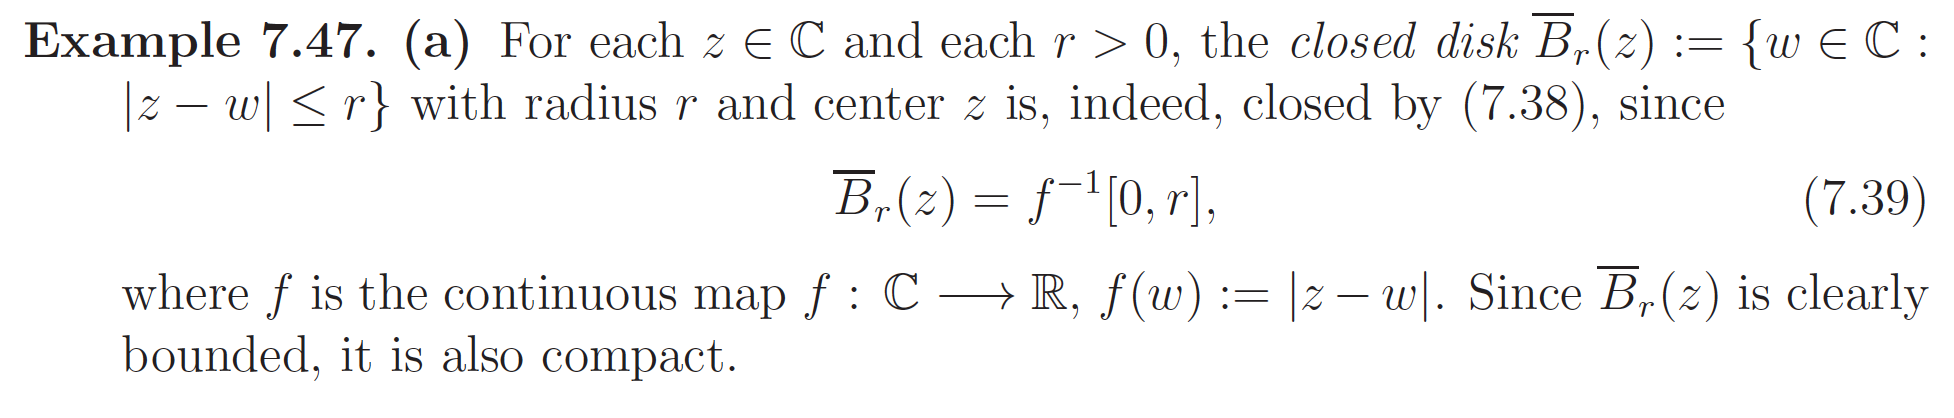
\includegraphics[width=0.7\textwidth]{media/7-14.png}
\end{figure}
\begin{figure}[H] \centering
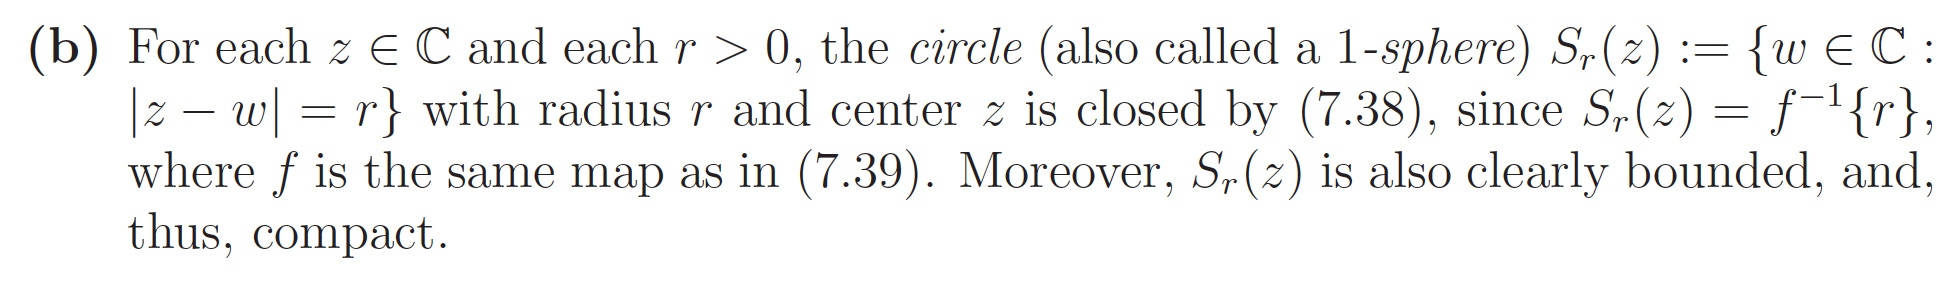
\includegraphics[width=0.7\textwidth]{media/7-14-2.png}
\end{figure}

\subsection{Halbräume in den komplexen Zahlen sind abgeschlossen. (82)}

\begin{figure}[H] \centering
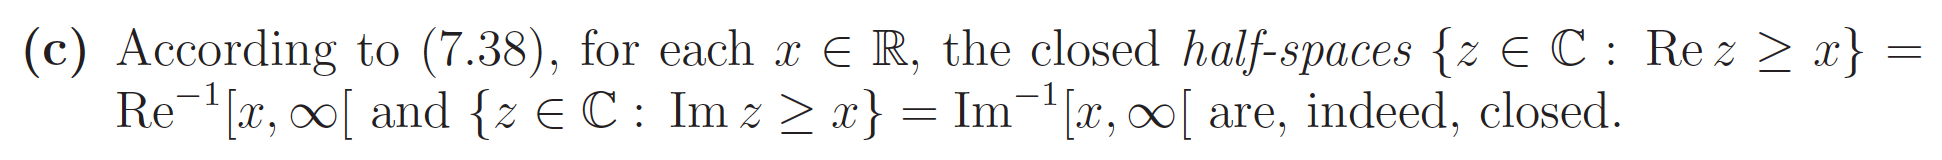
\includegraphics[width=0.7\textwidth]{media/7-15.png}
\end{figure}

\subsection{Satz: Stetige Bilder kompakter Mengen sind kompakt. (82)}

\begin{figure}[H] \centering
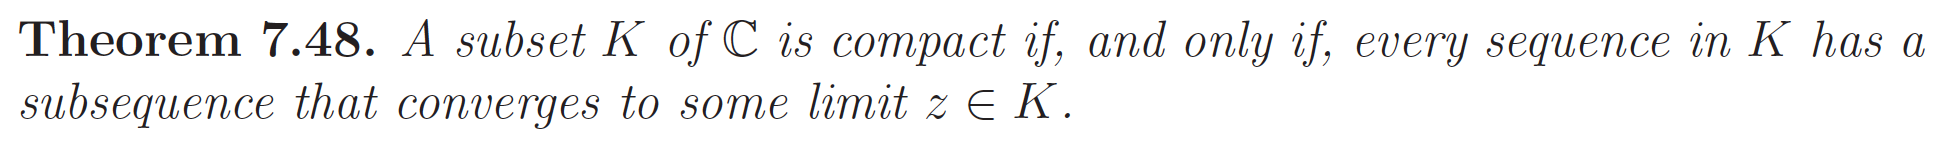
\includegraphics[width=0.7\textwidth]{media/7-16.png}
\end{figure}

\subsection{Definition globaler und lokaler Extrema ((strenge) Minima und Maxima). (82f)}

\begin{figure}[H] \centering
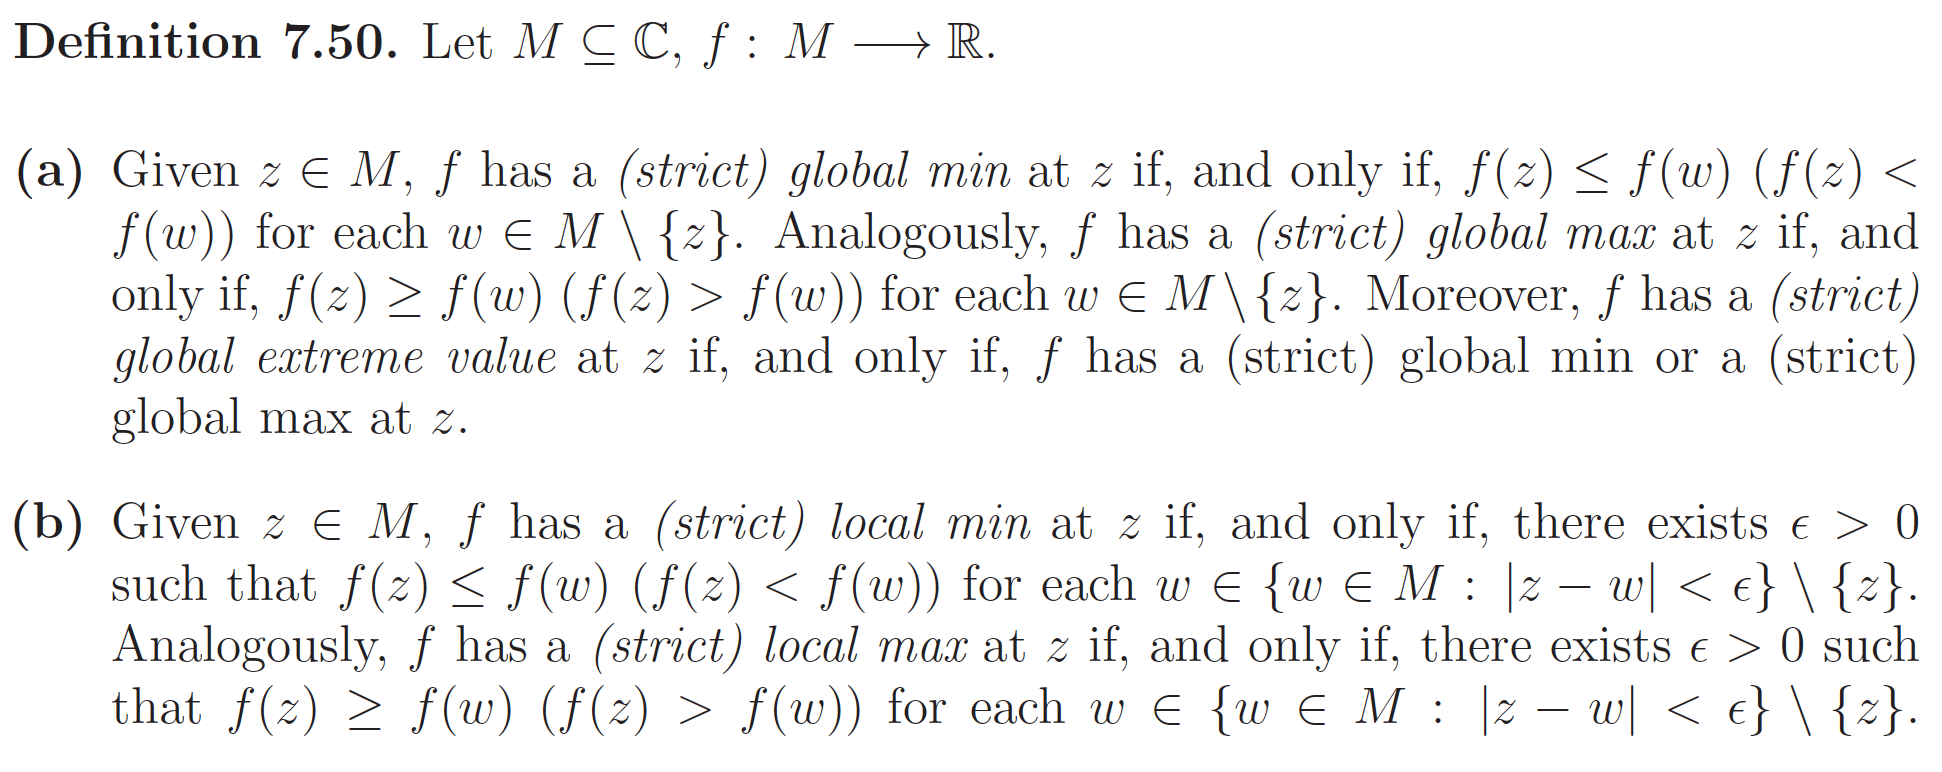
\includegraphics[width=0.7\textwidth]{media/7-17.png}
\end{figure}
\begin{figure}[H] \centering
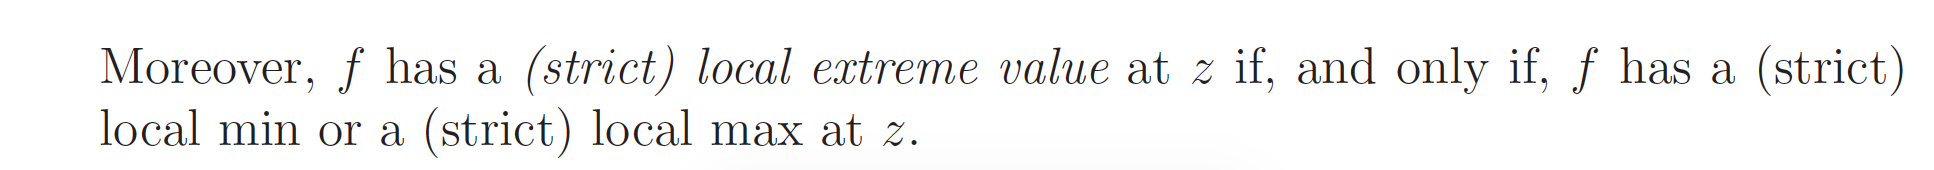
\includegraphics[width=0.7\textwidth]{media/7-17-2.png}
\end{figure}

\subsection{Satz: Stetige Abbildungen auf kompakten Mengen nehmen ihr (globales) Maximum und Minimum an.}

\begin{figure}[H] \centering
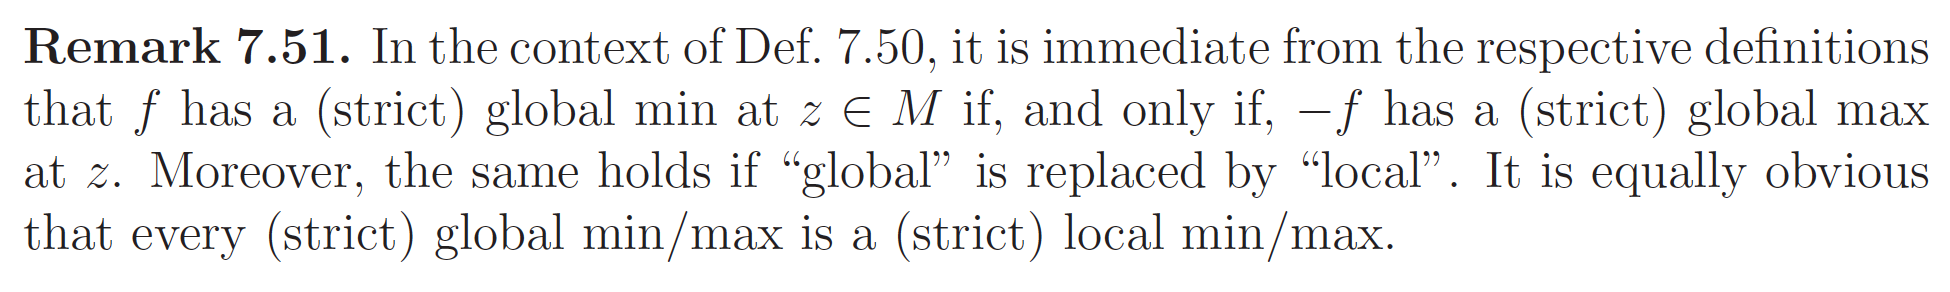
\includegraphics[width=0.7\textwidth]{media/7-18.png}
\end{figure}

\subsection{Nullstellensatz von Bolzano, Zwischenwertsatz, stetige Funktionen bilden Intervalle auf Intervalle ab. (84f)}

\begin{figure}[H] \centering
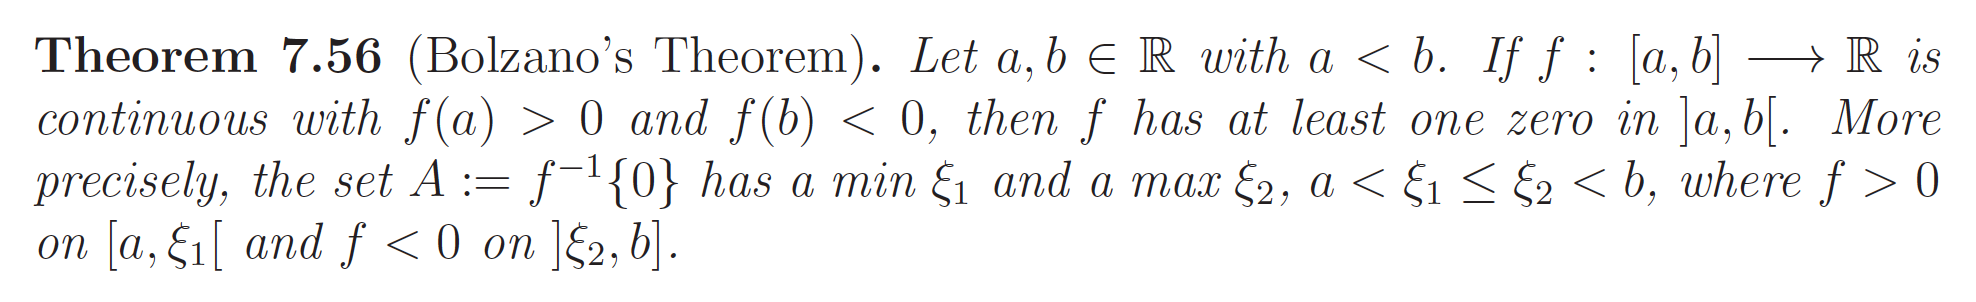
\includegraphics[width=0.7\textwidth]{media/7-19.png}
\end{figure}
\begin{figure}[H] \centering
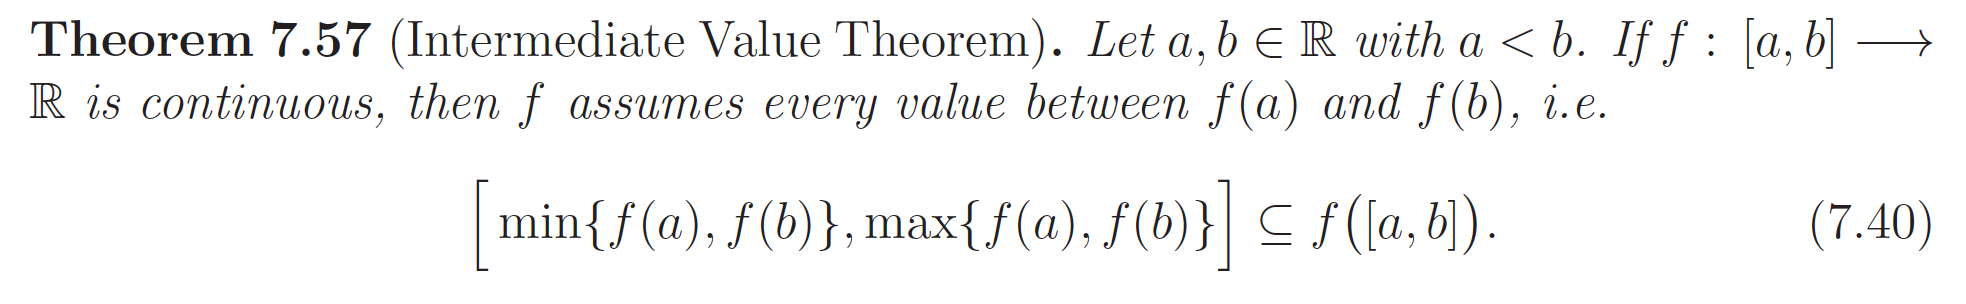
\includegraphics[width=0.7\textwidth]{media/7-19-2.png}
\end{figure}
\begin{figure}[H] \centering
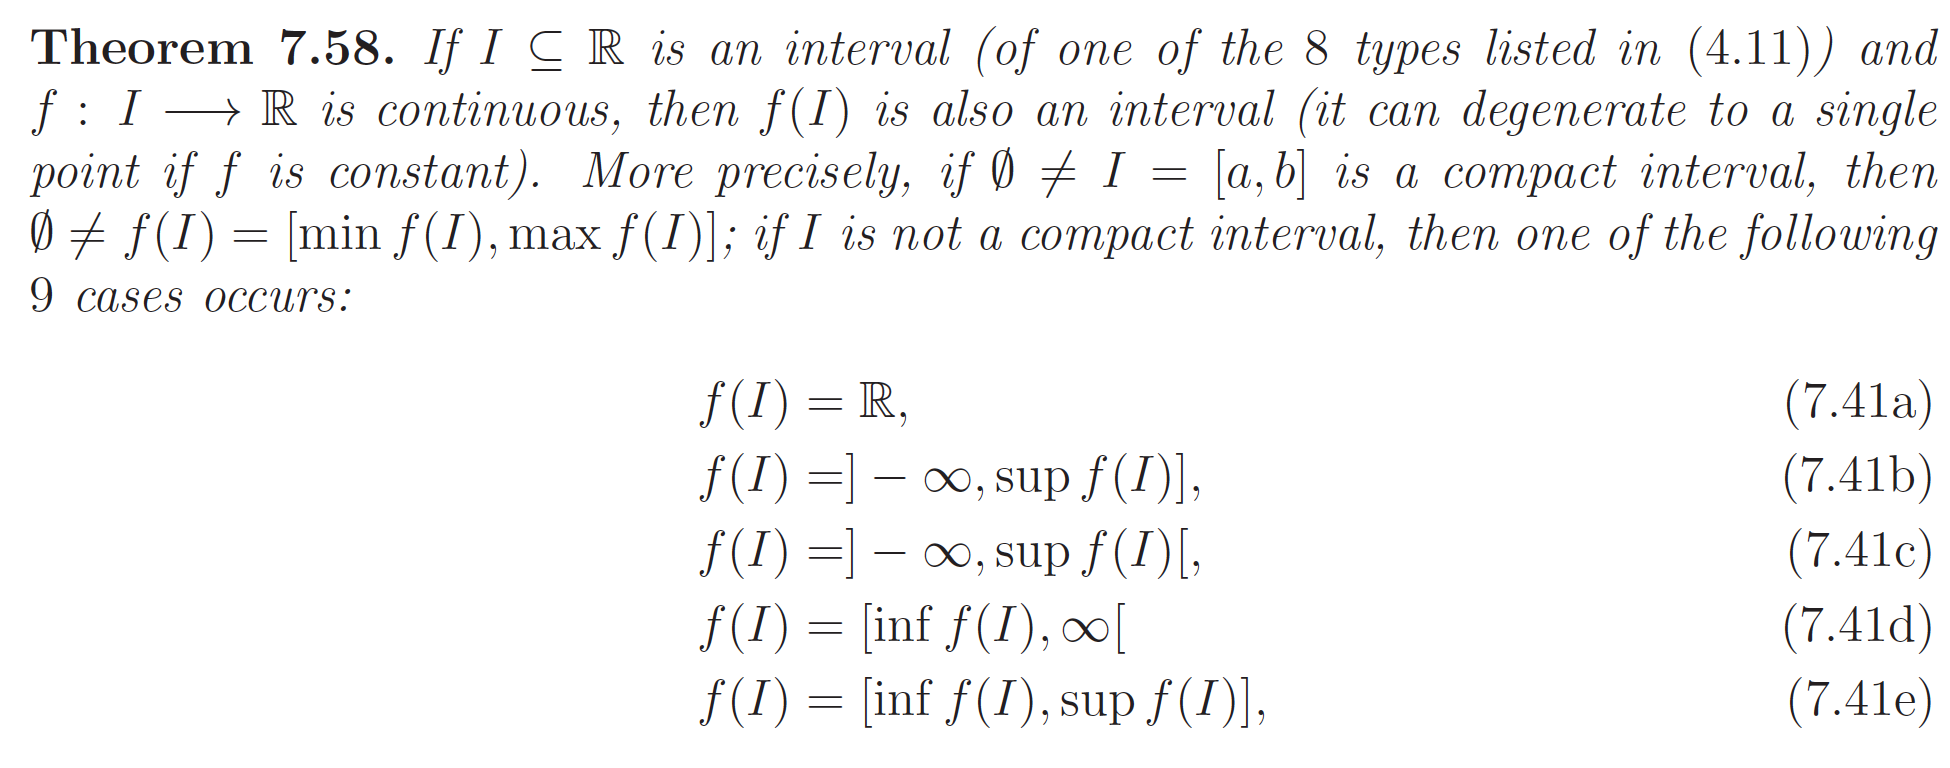
\includegraphics[width=0.7\textwidth]{media/7-19-3.png}
\end{figure}
\begin{figure}[H] \centering
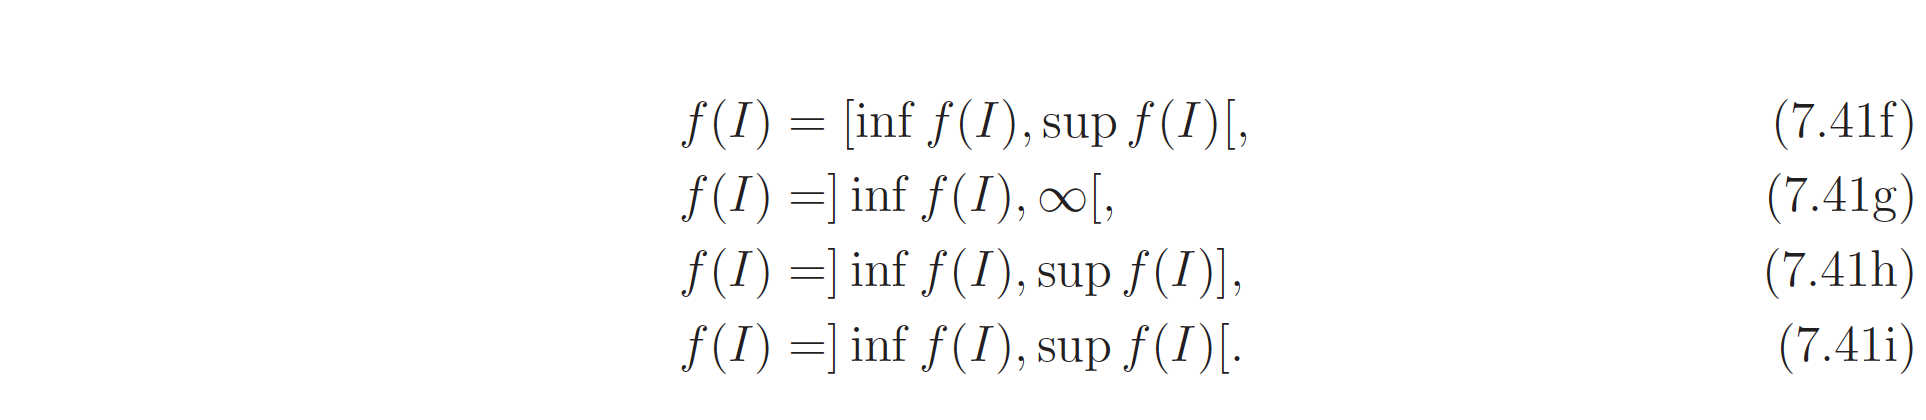
\includegraphics[width=0.7\textwidth]{media/7-19-4.png}
\end{figure}

\subsection{Definition der n.ten Wurzel einer nichtnegativen Zahl; die zugehörige Funktion ist stetig und streng monoton steigend. (86)}

\begin{figure}[H] \centering
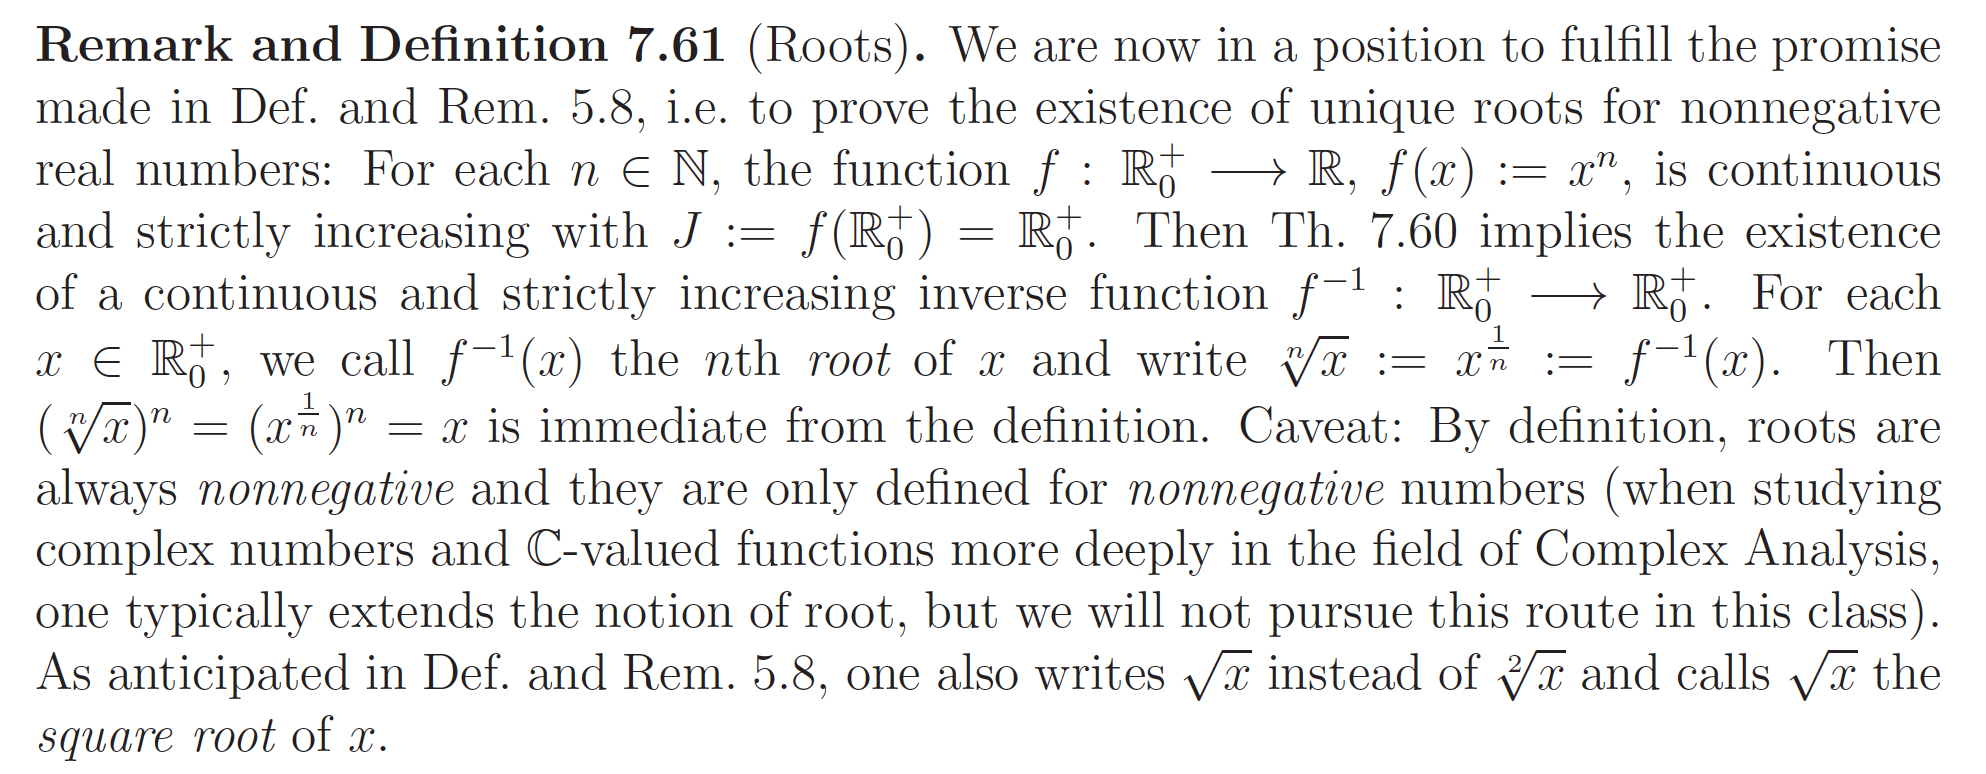
\includegraphics[width=0.7\textwidth]{media/7-20.png}
\end{figure}

\subsection{Nicht rationale Zahlen heißen irrational; die Menge der rationalen Zahlen ist abzählbar; die Menge der irrationalen Zahlen ist nicht abzählbar. (86)} 

\begin{figure}[H] \centering
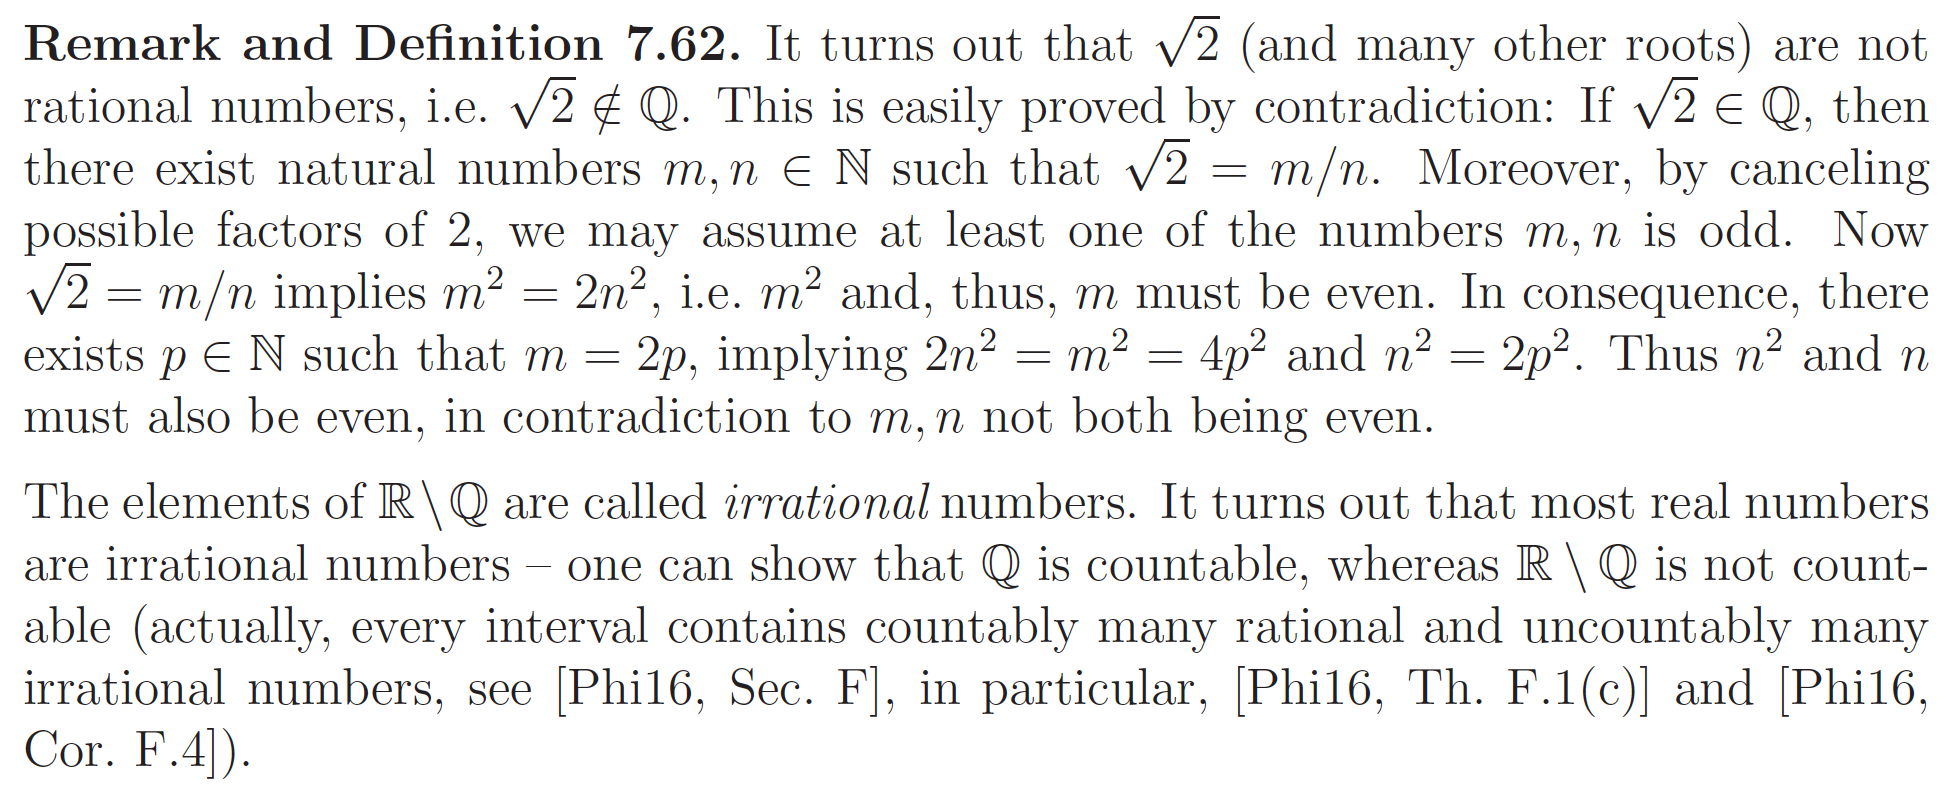
\includegraphics[width=0.7\textwidth]{media/7-21.png}
\end{figure}

\subsection{Definition der Dichtheit einer Menge in den reellen Zahlen. (88)}

\begin{figure}[H] \centering
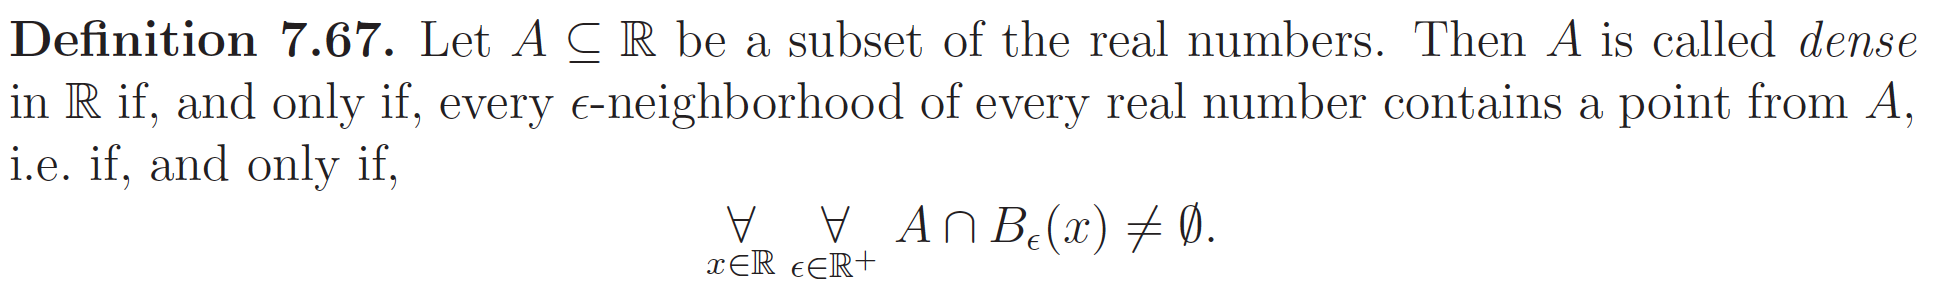
\includegraphics[width=0.7\textwidth]{media/7-22.png}
\end{figure}

\subsection{Satz: Die rationalen Zahlen sind dicht in den reellen Zahlen; die irrationalen Zahlen sind ebenfalls dicht. (88f)}

\begin{figure}[H] \centering
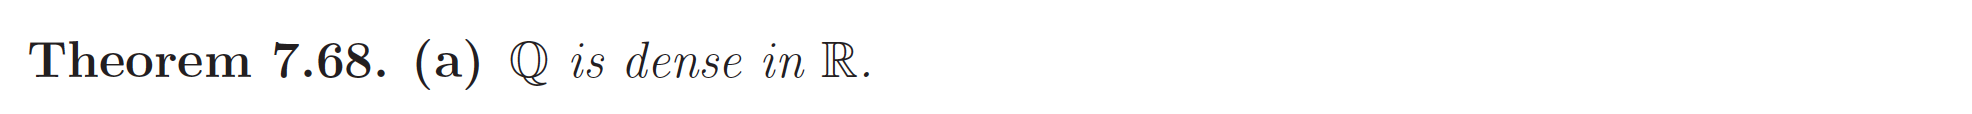
\includegraphics[width=0.7\textwidth]{media/7-23.png}
\end{figure}
\begin{figure}[H] \centering
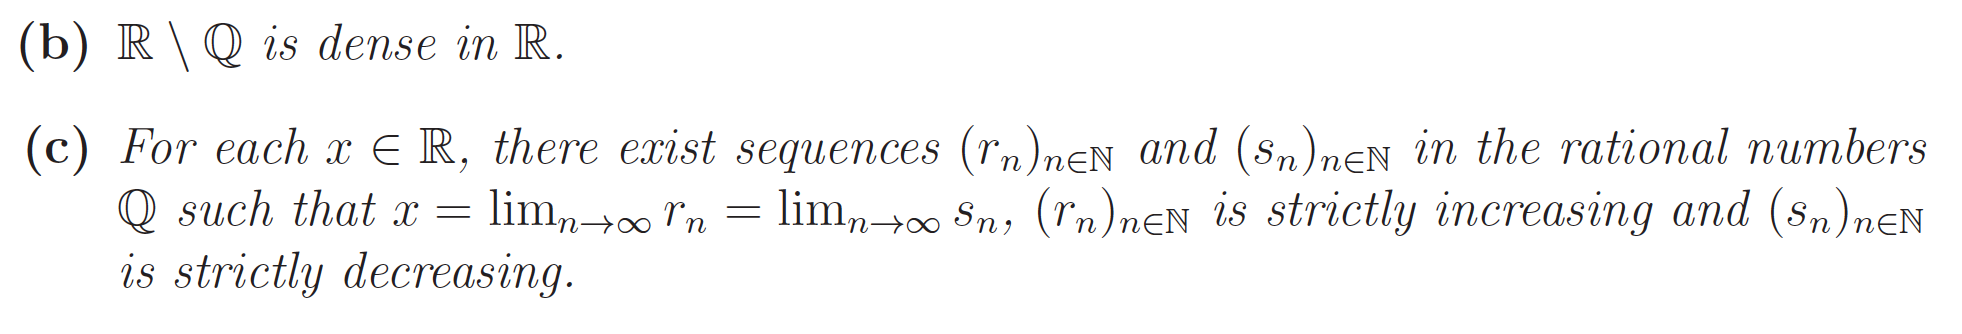
\includegraphics[width=0.7\textwidth]{media/7-23-2.png}
\end{figure}

\subsection{Satz: Jede reelle Zahl ist der Grenzwert einer streng steigenden Folge rationaler Zahlen und einer streng fallenden Folge rationaler Zahlen. (89)} 

\begin{figure}[H] \centering
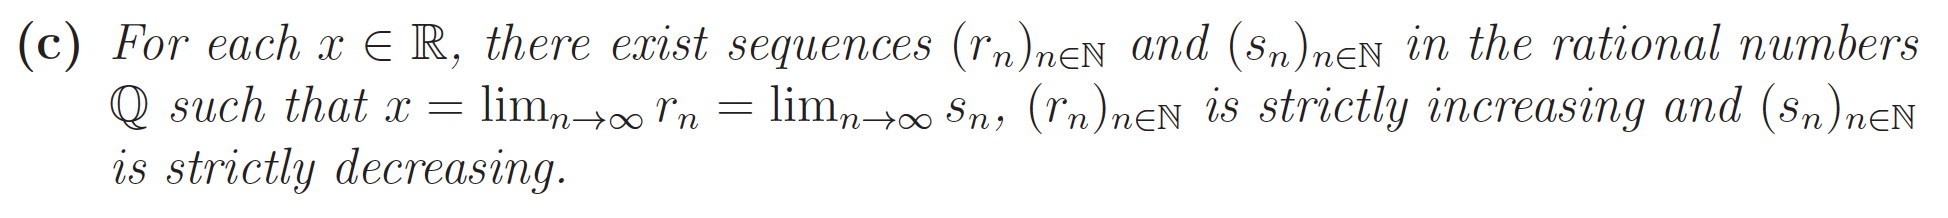
\includegraphics[width=0.7\textwidth]{media/7-24.png}
\end{figure}

\subsection{Definition von Potenzen mit nichtnegativer Basis und reellen Exponenten; es gelten die üblichen Potenzgesetze. (89f)}

\begin{figure}[H] \centering
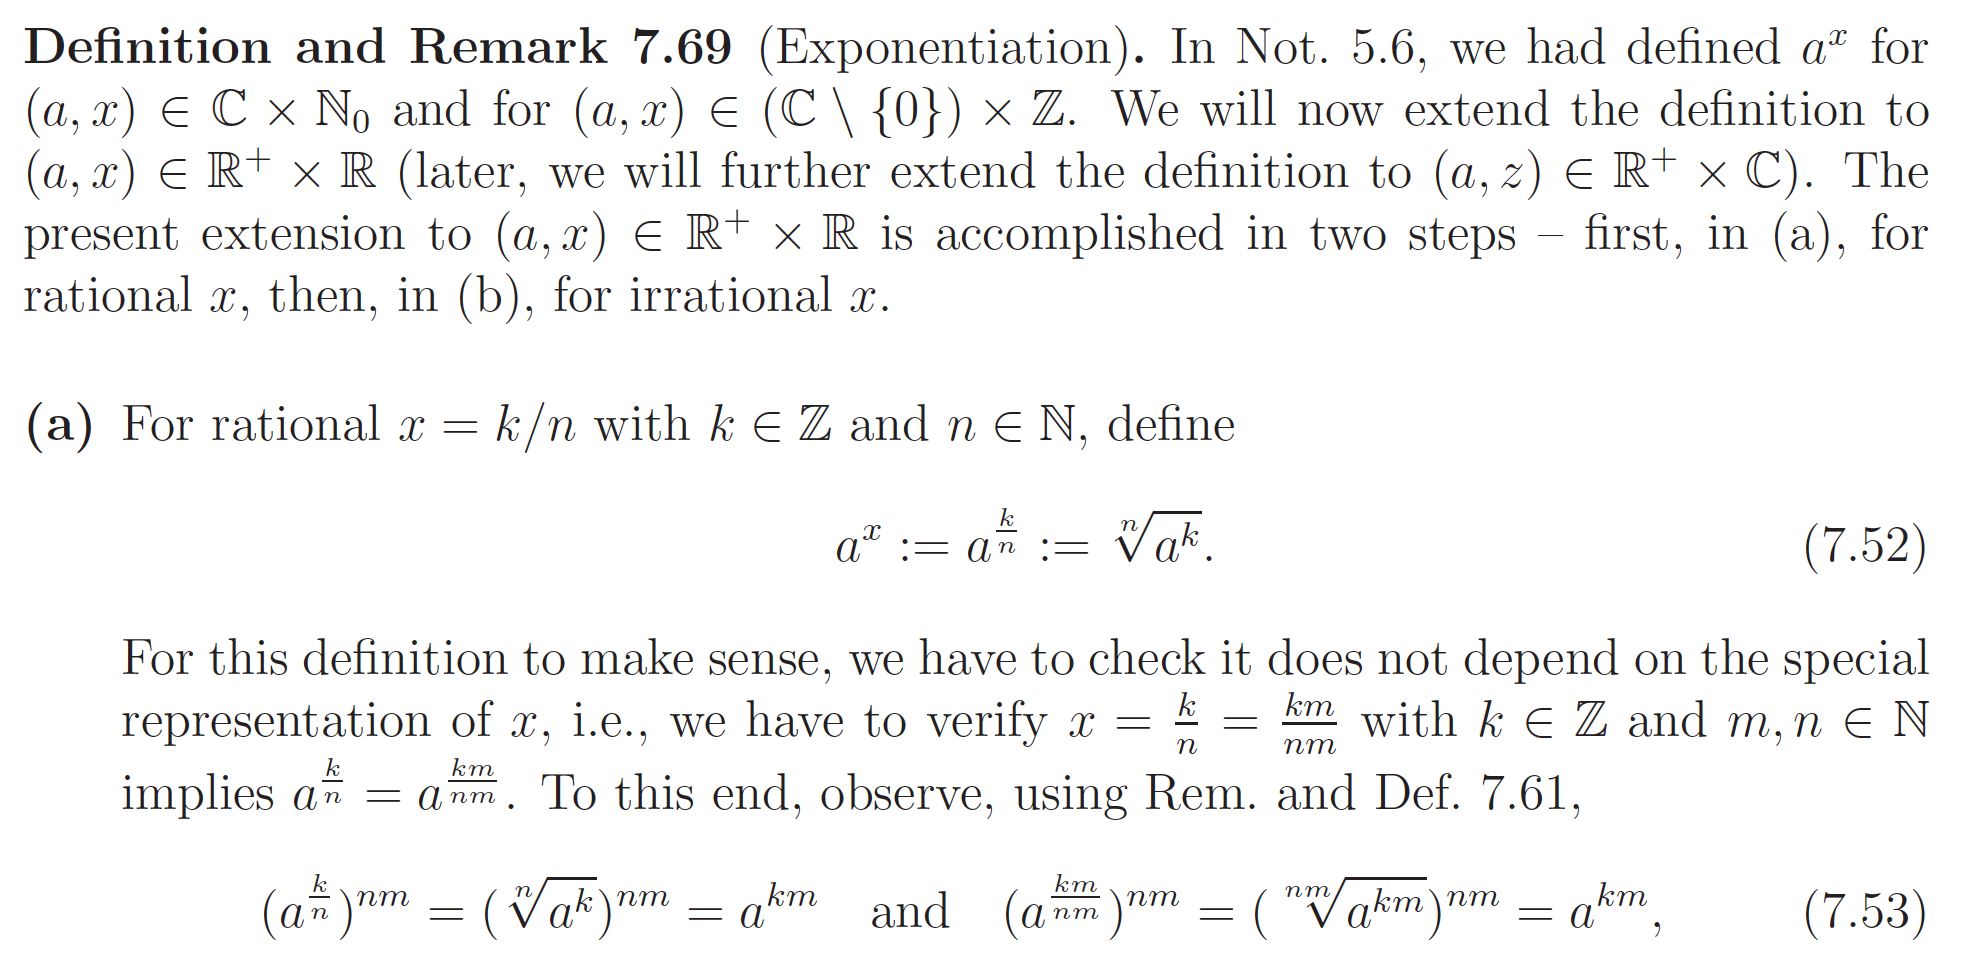
\includegraphics[width=0.7\textwidth]{media/7-25.png}
\end{figure}
\begin{figure}[H] \centering
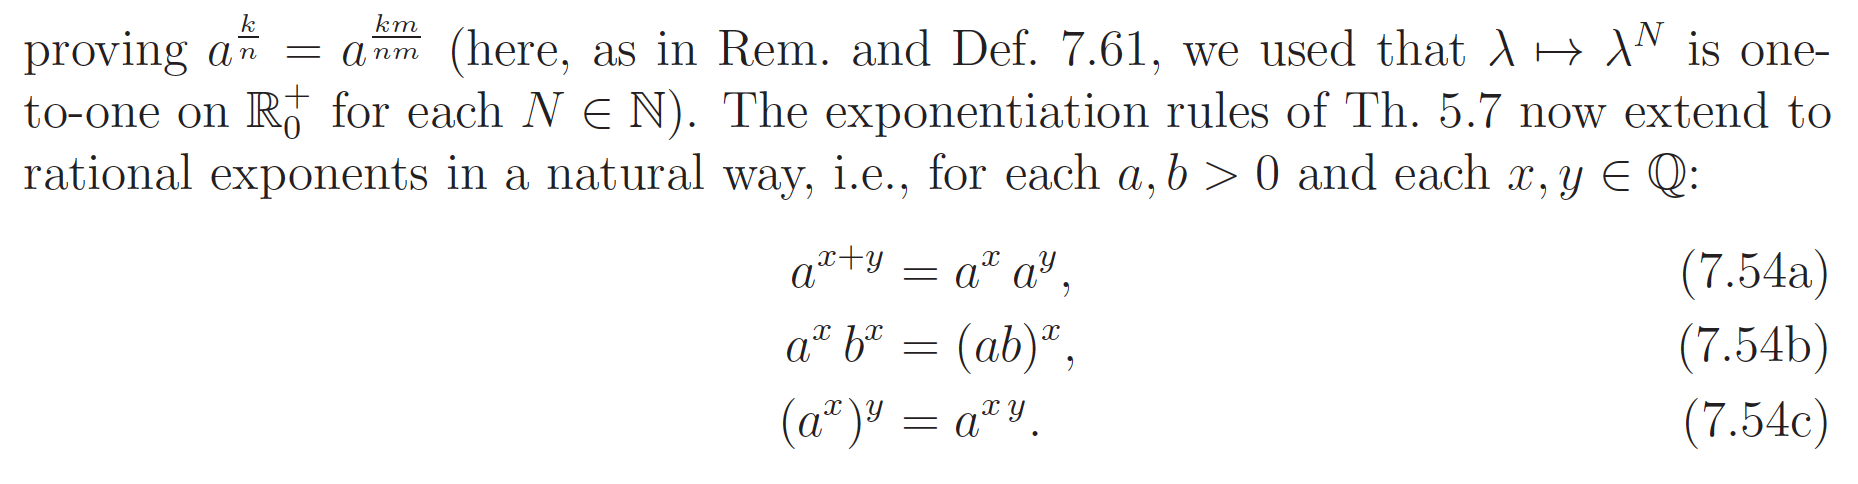
\includegraphics[width=0.7\textwidth]{media/7-25-2.png}
\end{figure}
\begin{figure}[H] \centering
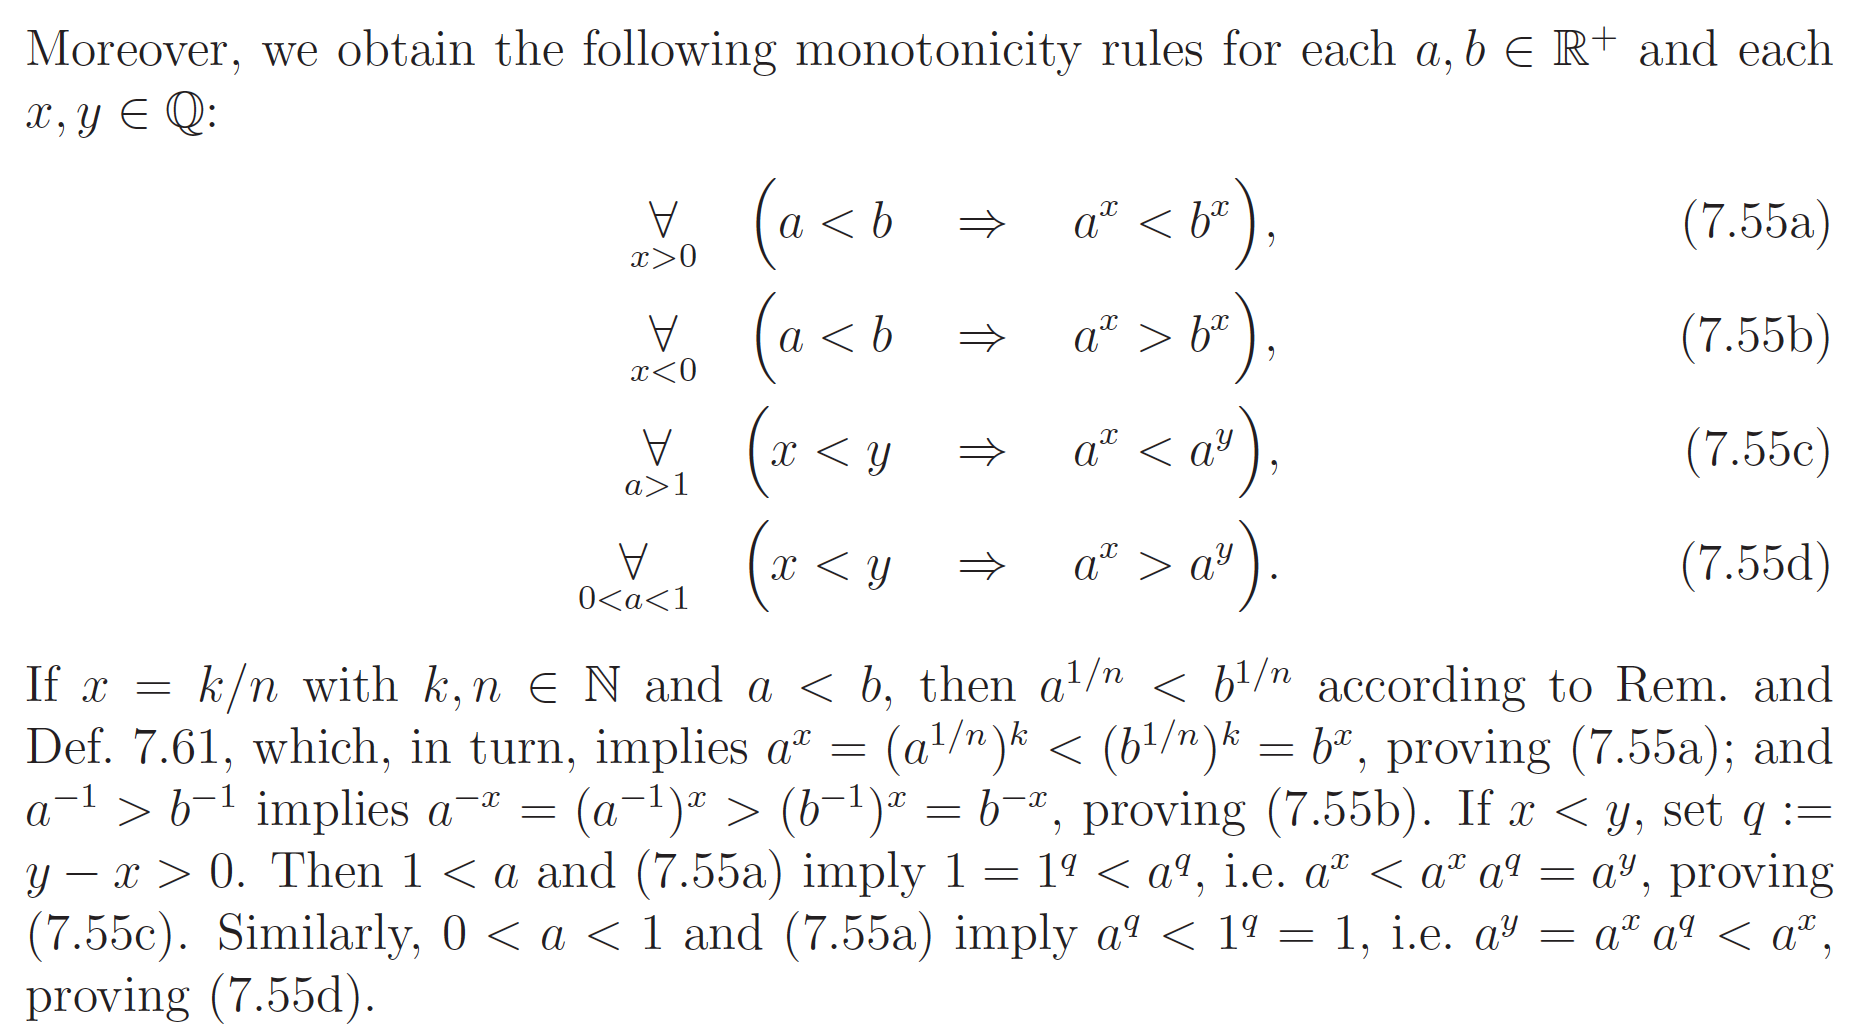
\includegraphics[width=0.7\textwidth]{media/7-25-3.png}
\end{figure}
\begin{figure}[H] \centering
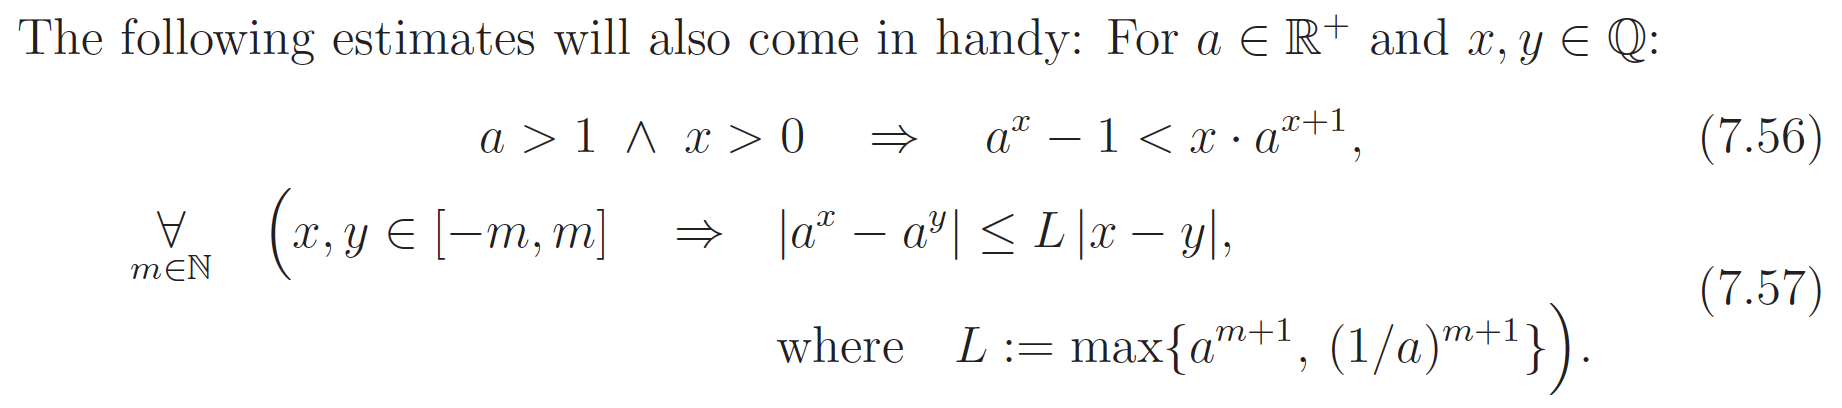
\includegraphics[width=0.7\textwidth]{media/7-25-4.png}
\end{figure}
\begin{figure}[H] \centering
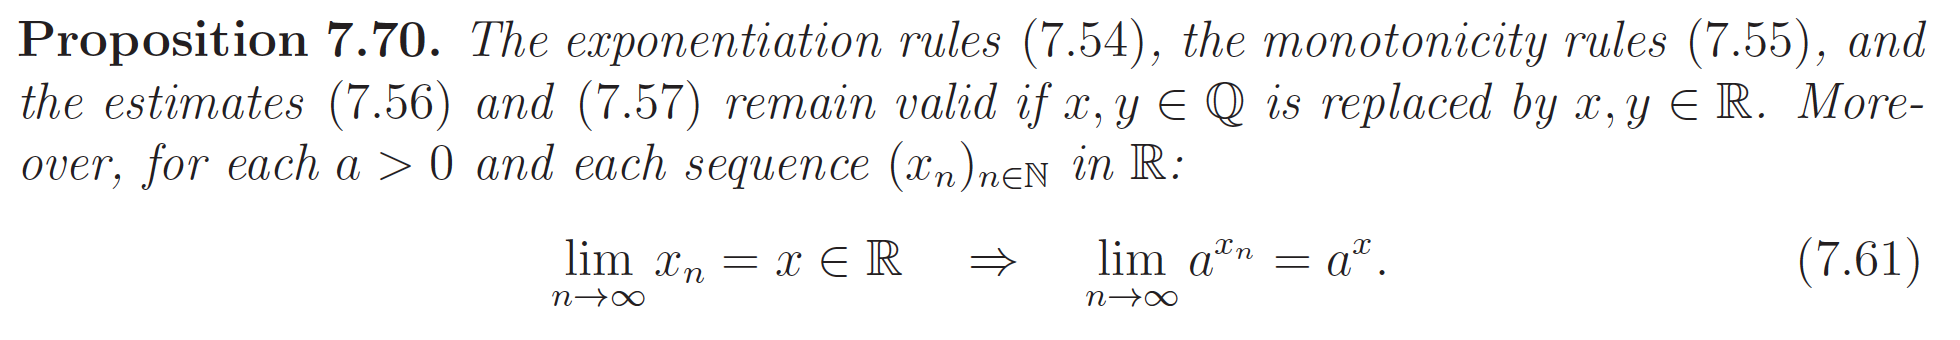
\includegraphics[width=0.7\textwidth]{media/7-25-5.png}
\end{figure}

\subsection{Definition von allgemeinen Potenzfunktionen und Exponentialfunktionen. (92)}

\begin{figure}[H] \centering
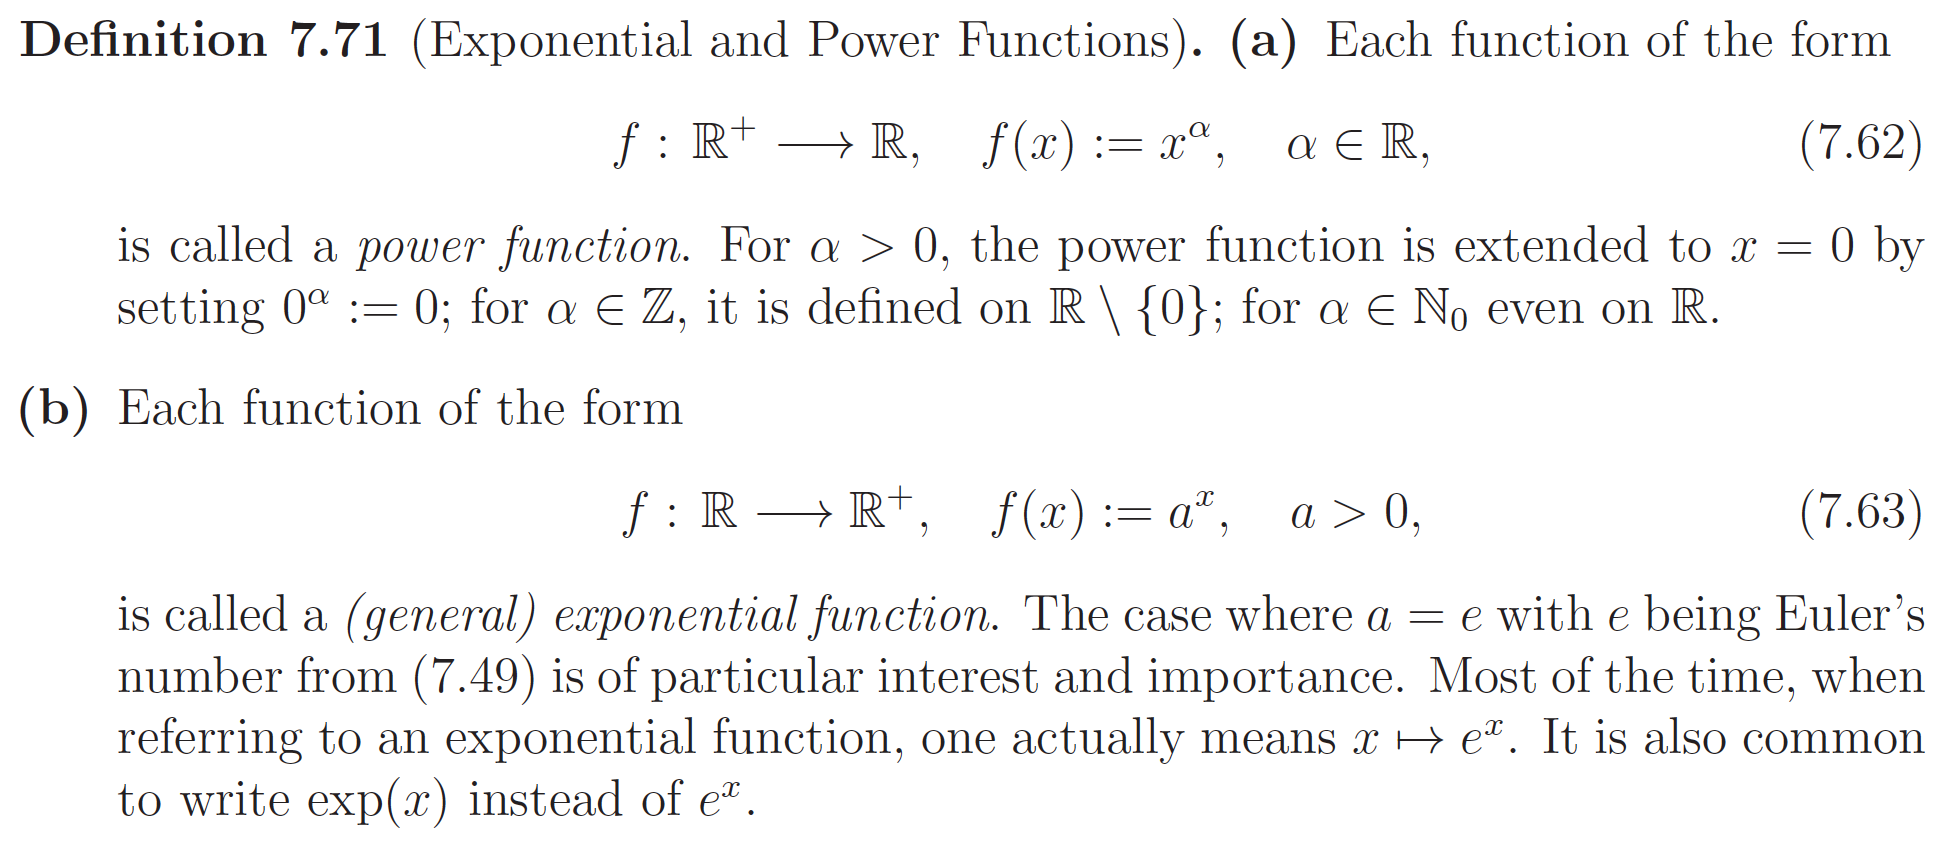
\includegraphics[width=0.7\textwidth]{media/7-26.png}
\end{figure}

\subsection{Satz: Potenzfunktionen sind auf ihrem jeweiligen Definitionsbereich stetig, sowie streng steigend für positiven und streng fallend für negativen Exponenten. (93)}

\begin{figure}[H] \centering
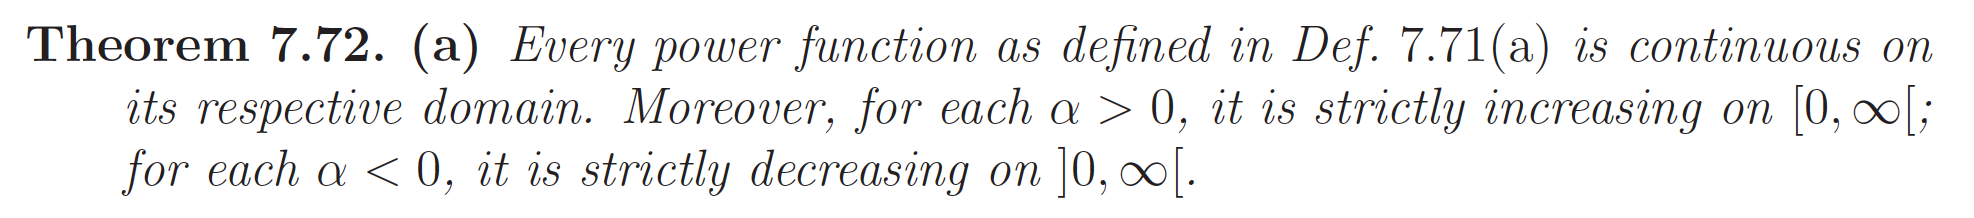
\includegraphics[width=0.7\textwidth]{media/7-27.png}
\end{figure}

\subsection{Satz: Exponentialfunktionen sind stetig sowie streng steigend für Basis a>1 und streng fallend für Basis 0 < a < 1. (93)}

\begin{figure}[H] \centering
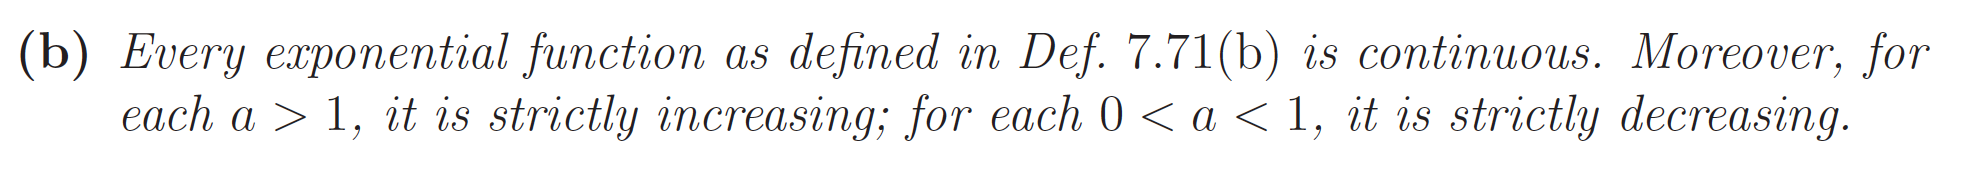
\includegraphics[width=0.7\textwidth]{media/7-28.png}
\end{figure}

\subsection{Definition des Logarithmus, speziell des natürlichen Logarithmus, Logarithmengesetze gemäß Th. 7.75. (93f)}

\begin{figure}[H] \centering
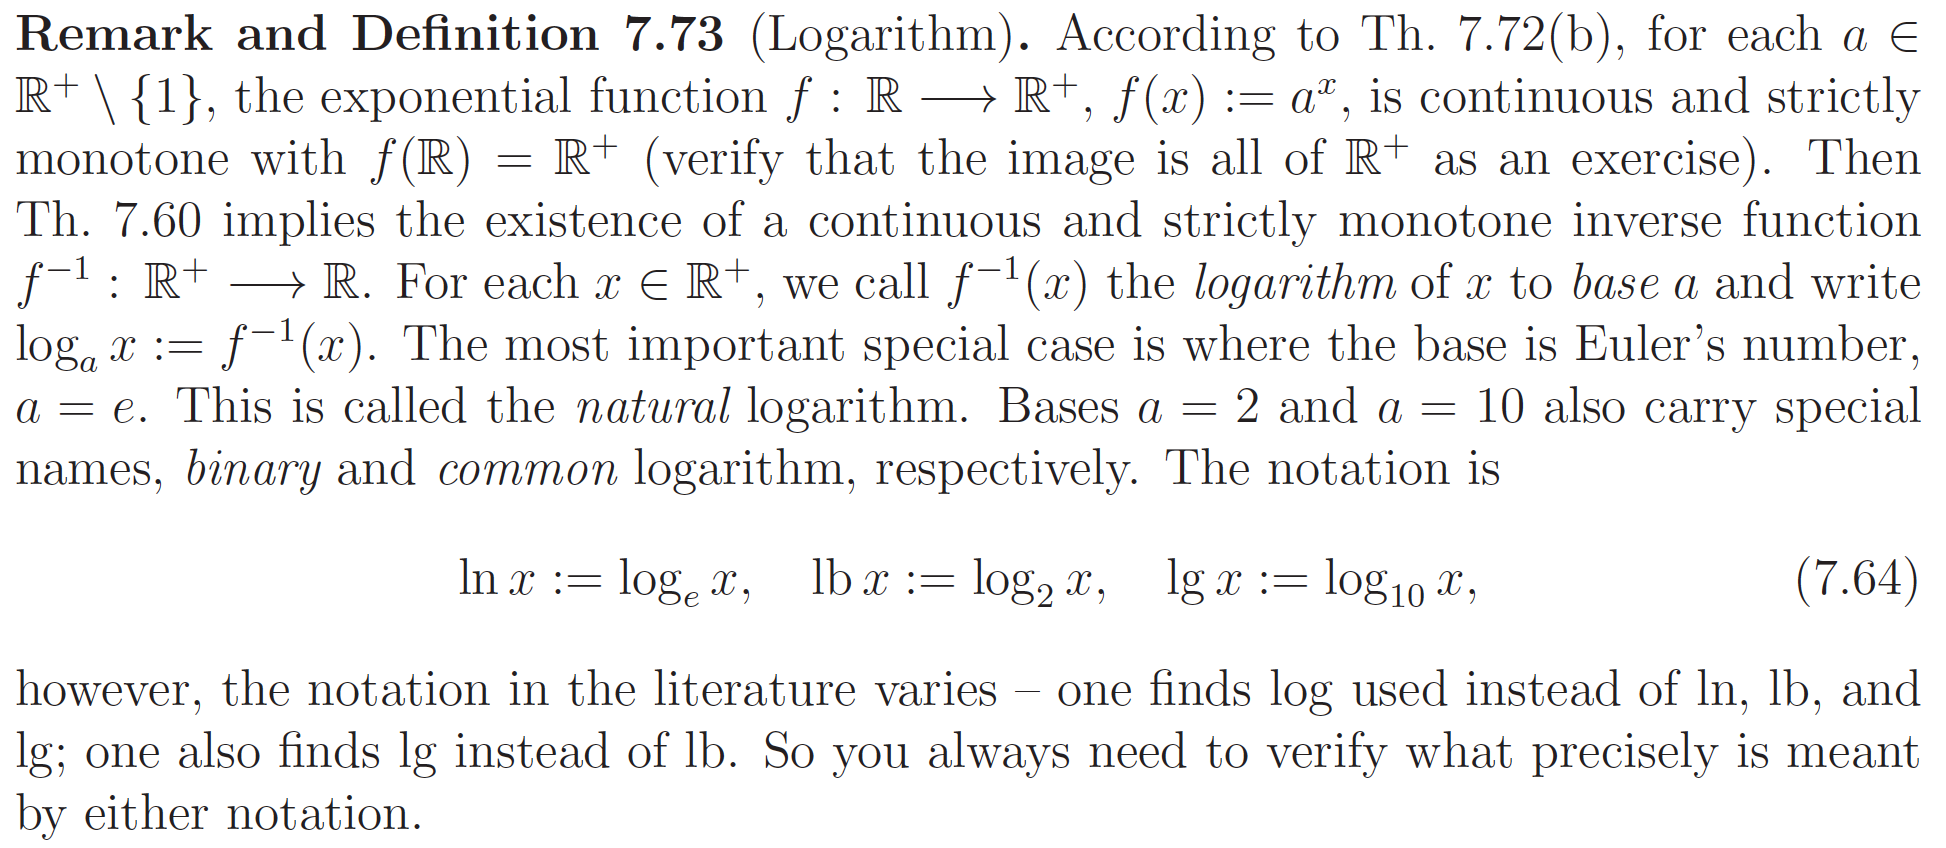
\includegraphics[width=0.7\textwidth]{media/7-29.png}
\end{figure}
\begin{figure}[H] \centering
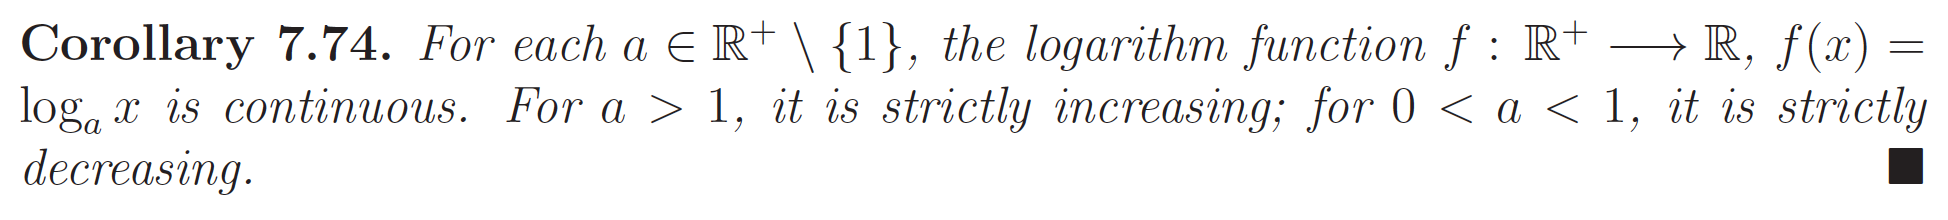
\includegraphics[width=0.7\textwidth]{media/7-29-2.png}
\end{figure}
\begin{figure}[H] \centering
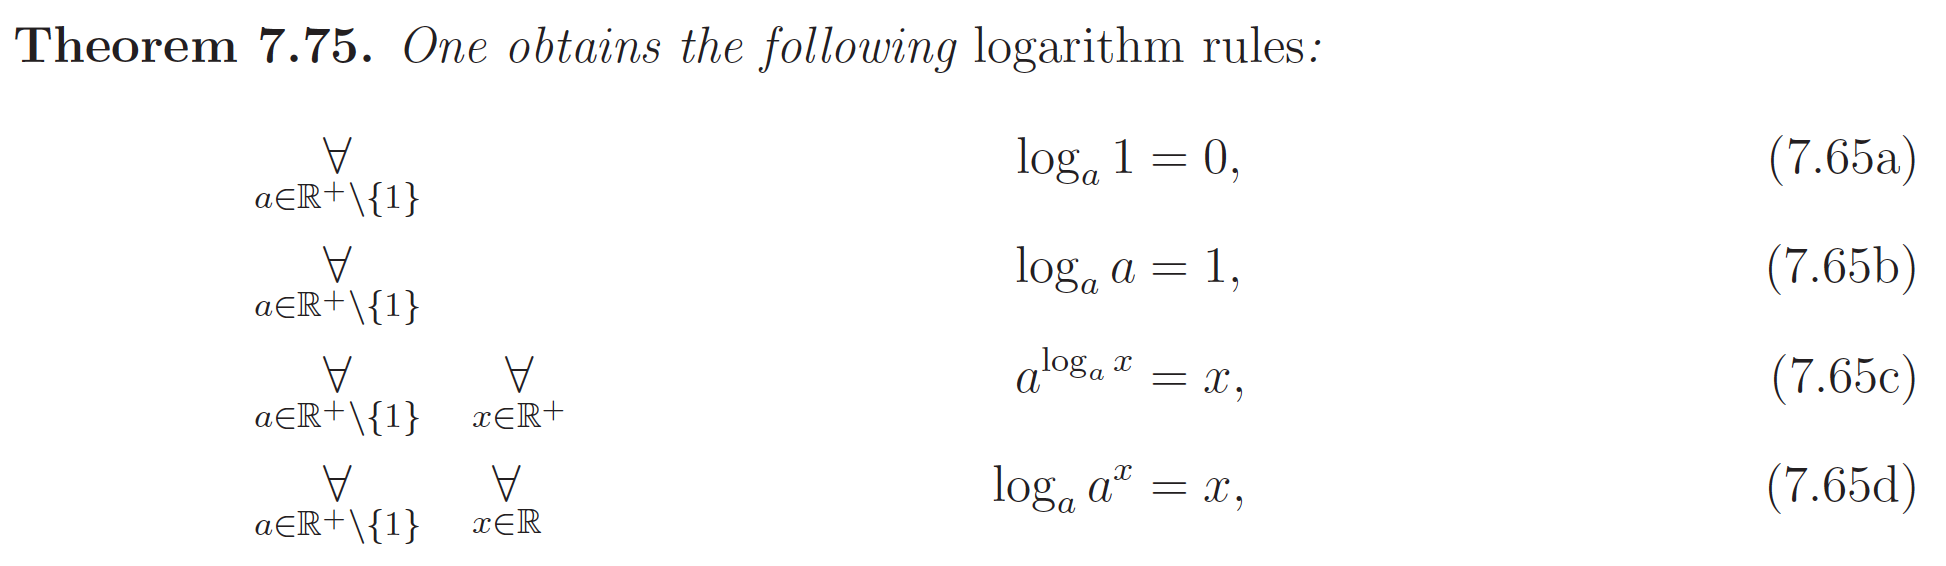
\includegraphics[width=0.7\textwidth]{media/7-29-3.png}
\end{figure}
\begin{figure}[H] \centering
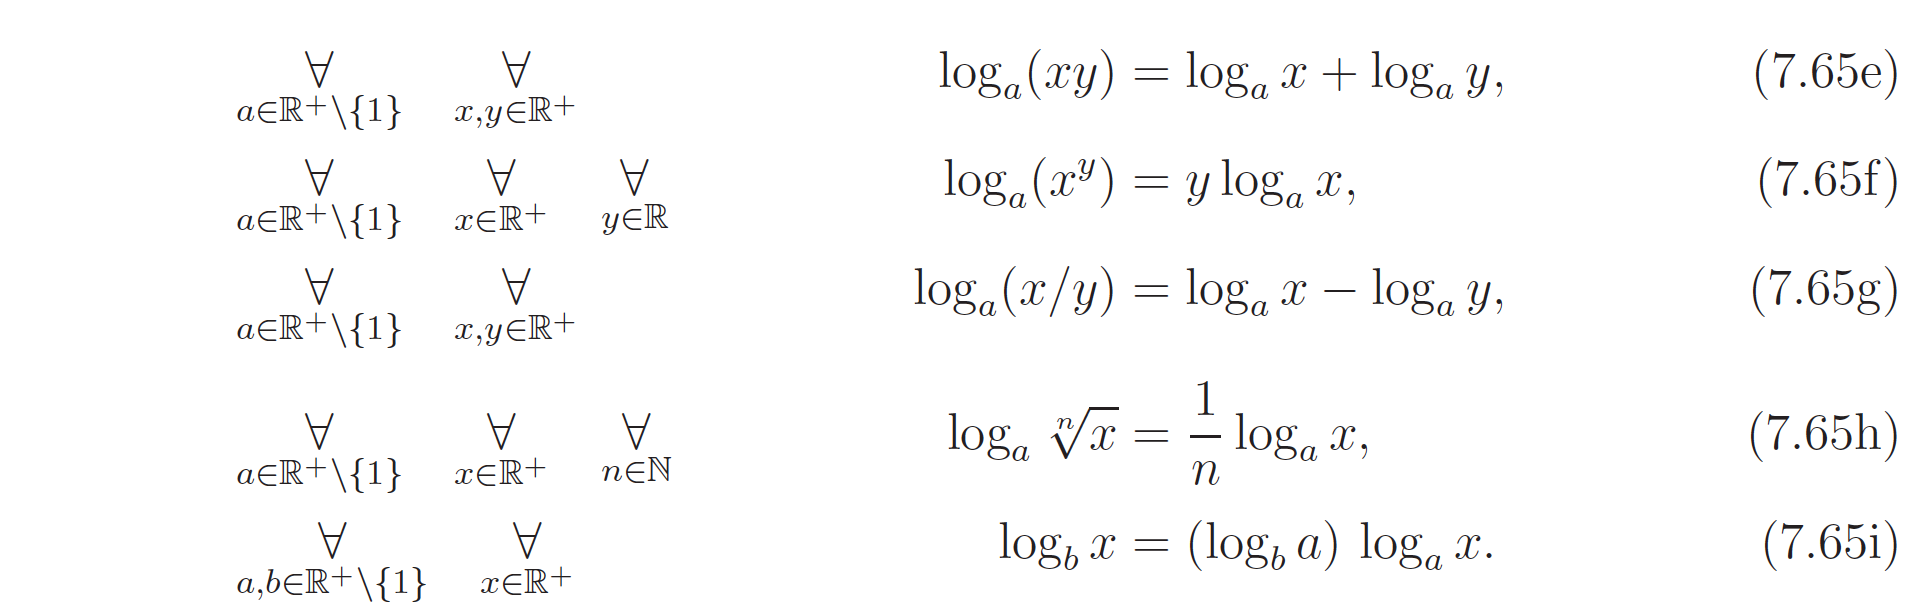
\includegraphics[width=0.7\textwidth]{media/7-29-4.png}
\end{figure}
\begin{figure}[H] \centering
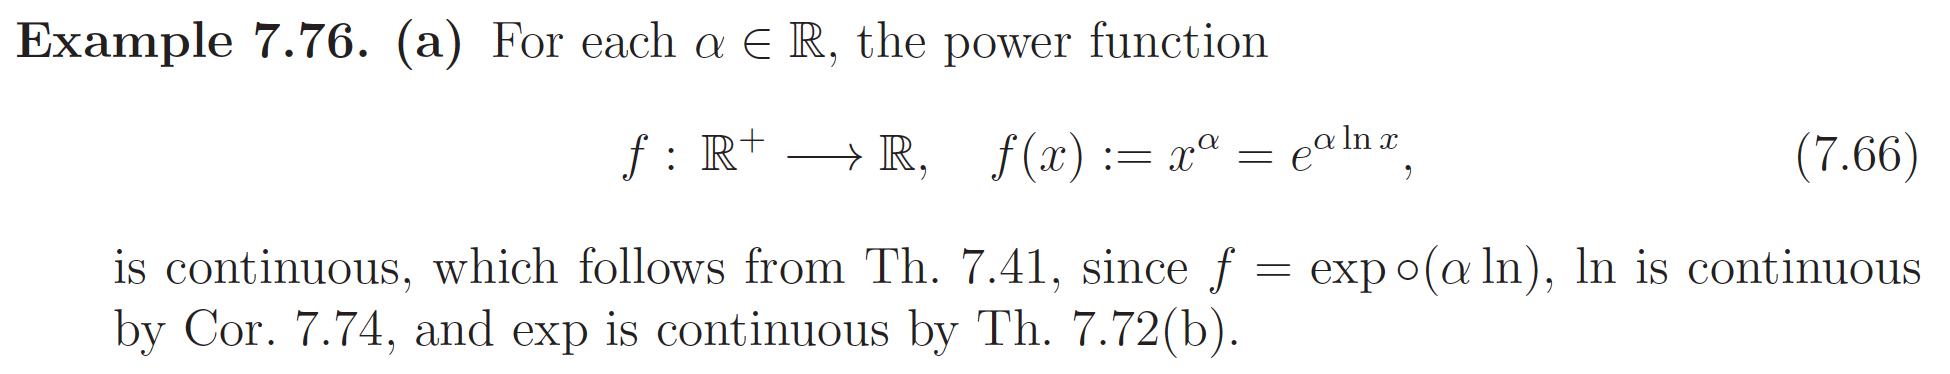
\includegraphics[width=0.7\textwidth]{media/7-29-5.png}
\end{figure}